\stepcounter{chapter} % This line will increment the chapter counter
\chapter*{Classification} % This line will create an unnumbered chapter
\addcontentsline{toc}{chapter}{\protect\numberline{\thechapter}Classification} % This line will add the chapter to your table of contents
\markboth{Classification}{} % This line will set the header
\vspace{-10mm}
This section contains the methods applied to two different classification problems: the first target chosen is the variable \texttt{genre}, which contains 20 different classes; next we tried to apply the same algorithms to \texttt{popularity}, a continuous variable discretized into three classes (low, medium, high). For this analysis, the data were standardized using \texttt{StandardScaler} (from \texttt{sklearn.preprocessing}), and in a first step we chose to use all features in the dataset before making a selection: \textit{explicit}, \textit{popularity}, \textit{danceability}, \textit{energy}, \textit{key} (one-hot encoded), \textit{loudness}, \textit{mode}, \textit{speechiness}, \textit{acousticness}, \textit{instrumentalness}, \textit{liveness}, \textit{valence}, \textit{tempo}, \textit{n\_bars}, \textit{processing}, \textit{genre}, \textit{duration\_min}. Which could be an expected accuracy value for the classification of \texttt{genre}? A starting point might be a comparison with a random model: a model that randomly assigns classes would have an expected accuracy of $5\%$ (1 in 20); therefore, any model with significantly higher accuracy than this could be considered an improvement, even if it did not achieve an accuracy close to 1. The same is true for classification with three classes, where any model with accuracy greater than 1/3 can be considered acceptable (for purely analytical purposes) although perhaps not realistically usable.\\
For each classification algorithm presented, the work process was carried out in several successive stages: initially we apply a basic model with default parameters by measuring its accuracy, so as to have a starting value to be improved with appropriate choice of parameters; in fact, the second stage concerns the tuning of the hyperparameters using \texttt{GridSearchCV} by \texttt{sklearn.model\_selection}; once the model with the optimal parameters is obtained, we proceed with the evaluation. All the analysis presented were performed on the entire dataset used for the previous steps, appropriately split into \texttt{train} and \texttt{test} subsets. For some further tests, an external test dataset (never seen by the models), provided by the lecturer, was also used in order to have the three sets train, validation and test.
\subsubsection*{Evaluation metrics and techniques}
\begin{itemize}
    \item \textsc{Accuracy and Overall Error Estimate}: fraction of predictions got right by our model and relative error (1-accuracy).
    \item \textsc{Precision-recall curves}: trade-off between the rate of true positives and the positive predictive value for a predictive model using different probability thresholds.
    \item \textsc{F1 score}: measures the performance of a model that combines precision and recall. It ranges from 0 to 1, where 1 indicates perfect precision and recall. 
    \item \textsc{ROC-AUC score}: performance of a classification model at all classification thresholds. The area under the curve (AUC) measures the 2D area under the ROC curve, providing an aggregate measure of performance across all classification thresholds.
\end{itemize}
All the results provided refer to the performance measure on the test set.
\newpage
\section{Target: \texttt{genre}}
\vspace{-0.5cm}
\subsection{KNN}
\begin{wrapfigure}{r}{0.4\textwidth}
\centering
\vspace{-2cm}
\caption{ROC-AUC and Precision/Recall for KNN model.}
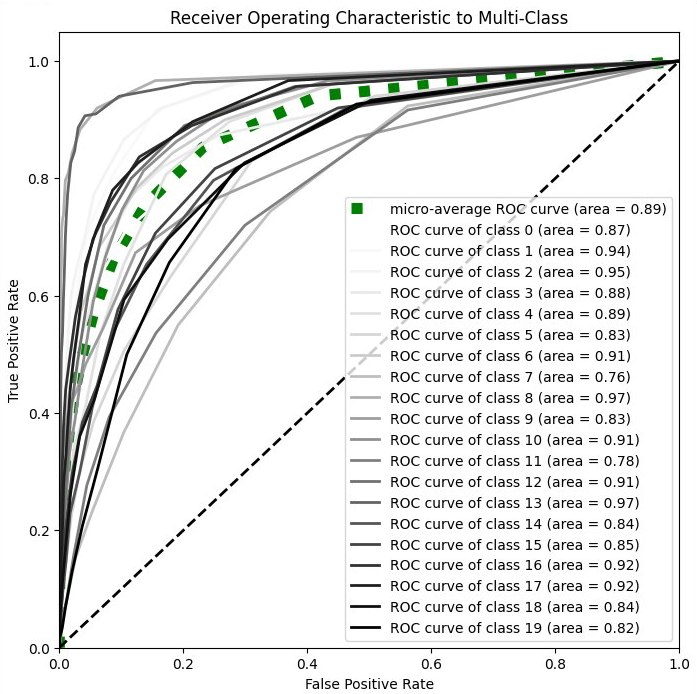
\includegraphics[width=0.8\linewidth]{img/roc_knn.jpg}
\vspace{2cm}
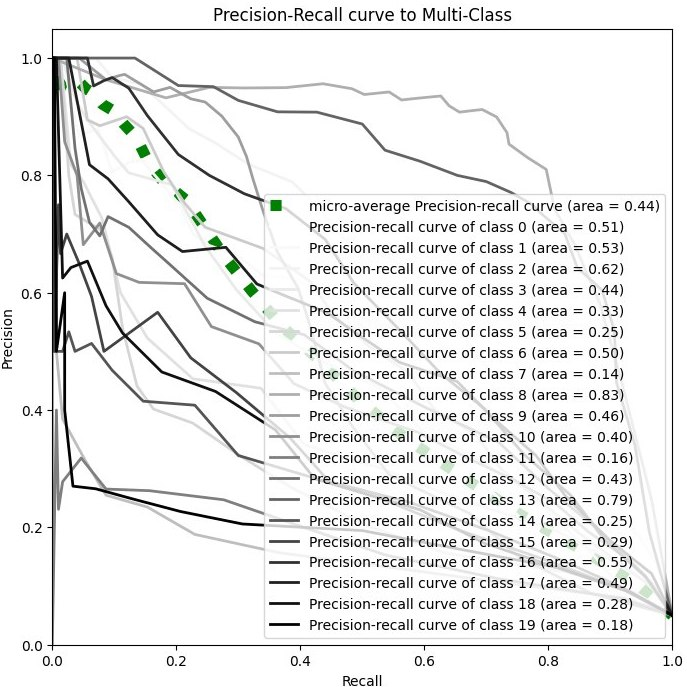
\includegraphics[width=0.8\linewidth]{img/pr_knn.jpg}
\vspace{-3cm}
\end{wrapfigure}

The base model returns an accuracy of $0.37$. For hyperparameter tuning, we start by looking at the trend of accuracy as the number of neighbors changes (from 1 to 100): the algorithm generates an error bar graph showing the average scores and their standard deviations for each number of neighbors and highlights the number of neighbors that obtained the highest accuracy, based on its cross-validation performance.
The configuration \texttt{\{'metric': 'cityblock', 'n\_neighbors': 26, 'weights': 'distance'\}} performs best according to GridSearch, with a final accuracy of about $0.48$.\\
\\
The model does not behave in the same way on the various classes, in particular it is better able to recognize tracks in the genre of "black metal" (class 2), "sleep" (class 8) and "study" (class 13).
\vspace{-0.5cm}
\subsection{Naive Bayes}
The Naive Bayes classifier is a classification algorithm based on Bayes' Theorem with the assumption that features are conditionally independent given the class label. In this study we distinctly use two types of NB: first, \texttt{Gaussian Naive Bayes}, a variant applicable to continuous variables in which attributes are assumed to follow a Gaussian distribution; it predicts the output variable based on each parameter independently. We then use \texttt{Categorical Naive Bayes}, suitable for discrete features that are categorically distributed.  
\begin{table}[H]
\centering
\footnotesize
\begin{tabular}{@{}|l|c|c|c|c|@{}}
\toprule
\rowcolor[HTML]{036400} 
{\color[HTML]{FFFFFF} \textbf{Classifier}} & \multicolumn{1}{l|}{\cellcolor[HTML]{036400}{\color[HTML]{FFFFFF} \textbf{Accuracy}}} & \multicolumn{1}{l|}{\cellcolor[HTML]{036400}{\color[HTML]{FFFFFF} \textbf{Precision}}} & \multicolumn{1}{l|}{\cellcolor[HTML]{036400}{\color[HTML]{FFFFFF} \textbf{Recall}}} & \multicolumn{1}{l|}{\cellcolor[HTML]{036400}{\color[HTML]{FFFFFF} \textbf{F1}}} \\ \midrule
\cellcolor[HTML]{C0C0C0}GaussianNB         & 0.37 & 0.37               & 0.37& 0.33                  \\ \midrule
\cellcolor[HTML]{C0C0C0}CategoricalNB & 0.40 & 0.38                           & 0.40 & 0.37                  \\ \bottomrule
\end{tabular}
\end{table}
\subsection{Decision Tree}
The base model returns a train accuracy of $1.0$ and a 
test accuracy $0.426$, with an obvious presence of overfitting. Before applying GridSearch we choose the ranges of some parameters based on the behavior of the model by plotting accuracy against different values: in particular we tuned \texttt{max\_depth}, \texttt{min\_samples\_split} and \texttt{min\_samples\_leaf}. The configuration with the optimal parameters turns out to be \texttt{\{'splitter': 'best', 'min\_samples\_split': 56, 'min\_samples\_leaf': 10, 'max\_depth': 11, 'criterion': 'gini'\}}, with an average accuracy of $0.45$. To visualize the tree we used \texttt{tree.export\_graphviz} from \texttt{sklearn} (below the graph is cut down to $\texttt{max\_depth}=2$ to make its content more understandable).
\begin{figure}[H]
    \centering
    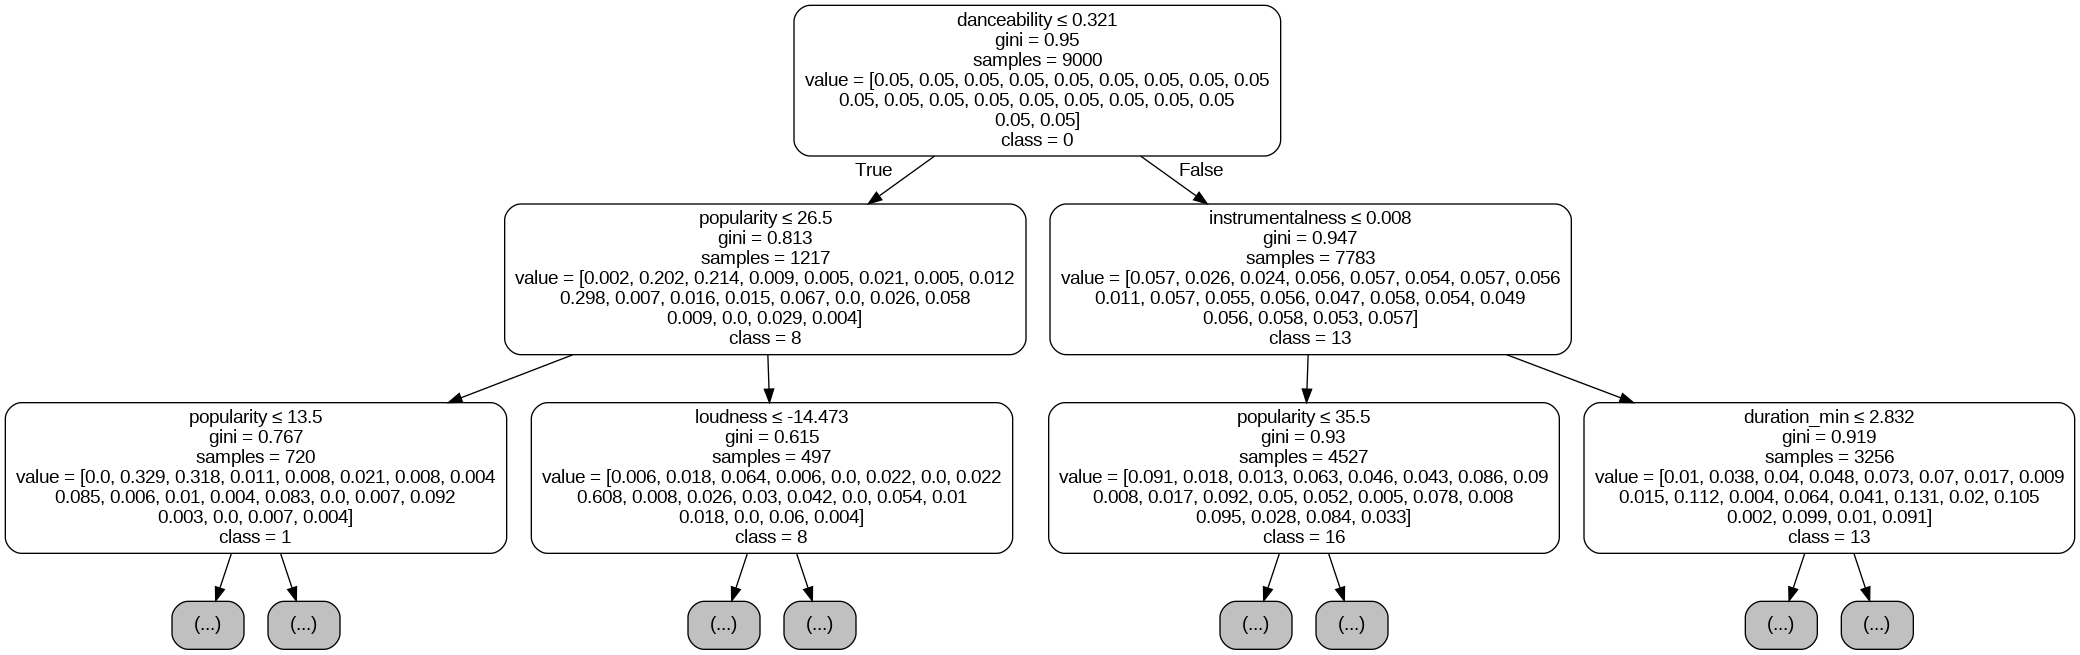
\includegraphics[scale=0.2]{img/decision_tree_genre_graphviz.png}
    \caption{Decision Tree with \texttt{genre} as target variable.}
    \label{fig:enter-label}
\end{figure}
\noindent We can also see the importance of features according to the model used: the most important is \texttt{popularity} ($0.23$), followed by \texttt{acousticness} ($0.13$), \texttt{danceability} ($0.13$), \texttt{duration\_min} ($0.12$) and so on; along with some features that have a very low contribution (like \texttt{liveness} or \texttt{processing}), we see that \texttt{key}, \texttt{explicit} and \texttt{mode} result useless (according to this model) in determining the genre of the track. We can therefore assume that the model relies mainly on how popular, acoustic and danceable a track is to identify its genre. Although predicting genre using popularity might be counterintuitive, removing it from features drops performance dramatically.\\ In a Decision Tree, when the parameter \texttt{ccp\_alpha} increases, more of the tree is pruned, thus creating a decision tree that generalizes better. So we implemented a procedure that could find the optimal value of the parameter. The result is [\texttt{Best ccp\_alpha value is:  0.000386}], but the performance of the model has not improved noticeably (accuracy about $0.46$).\\
We anticipated above that for an initial classification study we used all the features in the dataset. After seeing how all the models behaved, we decided to make a selection of the variables to be used: we used the correlation coefficient (the highest the correlation with target the highest the importance) and \texttt{mutual\_info\_classif} from \texttt{sklearn.feature\_selection}, that measures the reduction in entropy about one variable given the knowledge of another; in other words, it measures the dependency between each feature and the target variable. We used these two tools to obtain a combined score of each variable, so that we could select those with the highest score. From the results comes confirmation of the features identified by the decision tree; in fact, by selecting the 5 features with the highest score, we can repeat the analysis using only the variables \texttt{danceability}, \texttt{popularity}, \texttt{acousticness}, \texttt{energy}, \texttt{valence}. To recapitulate, the overall results are:
\begin{table}[H]
\centering
\footnotesize
\begin{tabular}{|l|c|c|c|c|c|}
\hline
\rowcolor[HTML]{036400} 
{\color[HTML]{FFFFFF} Decision Tree}      & {\color[HTML]{FFFFFF} Train acc} & {\color[HTML]{FFFFFF} Test acc} & {\color[HTML]{FFFFFF} precision} & {\color[HTML]{FFFFFF} recall} & {\color[HTML]{FFFFFF} F1} \\ \hline
\cellcolor[HTML]{C0C0C0}base model        & 1.0                              & 0.43                            & 0.43                             & 0.43                          & 0.43                      \\ \hline
\cellcolor[HTML]{C0C0C0}GridSearch        & 0.55                             & 0.45                            & 0.47                             & 0.46                          & 0.46                      \\ \hline
\cellcolor[HTML]{C0C0C0}ccp\_alpha        & 0.55                             & 0.46                            & 0.47                             & 0.46                          & 0.46                      \\ \hline
\cellcolor[HTML]{C0C0C0}Feature selection & 0.54                             & 0.46                            & 0.47                             & 0.46                          & 0.46                      \\ \hline
\end{tabular}
\end{table}
\subsection{Results}
\begin{itemize}
    \item KNN: [\texttt{accuracy}: $0.48$, \texttt{roc auc}: $0.89$, \texttt{precision/recall auc}: $0.44$]. Although we have improved the basic model and we are above the expected value of an accuracy of $1/20$, for pure analytical purposes we can consider the model acceptable but not usable in a real-world context, given the high error rate: about half of the data are not classified correctly.
    \item Naive Bayes: In this case the error increases to about $60\%$, which means that the two models Gaussian and Categorical (on different feature groups, continuous and categorical) still perform worse than KNN.
    \item DecisionTree: The accuracy of the model does not exceed $0.46$, even after appropriate parameter tuning. However, we can still study the behavior of the model and how it was able to capture relationships between variables based on the importance given in the training phase.
\end{itemize}
\section{Target: \texttt{popularity}}
As anticipated, we also decided to test the studied techniques on another target variable: we discretized popularity using \texttt{pd.cut} into three classes, \texttt{[Low (0-50), Medium (50-80), High (80-100)]}. We followed the same process used for the target \texttt{genre}, that is, we started with a basic model (for this study we used only the Decision Tree) and then tuned its parameters to improve its performance. In this case, the optimal configuration is \texttt{\{'splitter': 'best', 'min\_samples\_split': 94, 'min\_samples\_leaf': 58, 'max\_depth': 5, 'criterion': 'entropy'\}} with an average accuracy of $0.87$. The most important features are \texttt{genre}, \texttt{energy} and \texttt{instumentalness}.\\ In this case, however, there is a problem of class imbalance: in fact, tracks with low popularity cover almost the entire dataset, mediums are on the order of hundreds, and highs are a few dozen. So we implemented a process for optimizing class weights in the classifier, in order to handle class imbalance. The code generates a range of weights for the classes, calculates 10-fold cross-validated F1 scores for each set of weights, identifies the weights that yield the highest score, and trains a final model using these optimal weights. We then again applied the procedure for the ccp\_alpha parameter and feature selection. The results are:
\begin{table}[H]
\centering
\footnotesize
\begin{tabular}{|l|c|c|c|c|c|}
\hline
\rowcolor[HTML]{036400} 
{\color[HTML]{FFFFFF} Decision Tree}      & {\color[HTML]{FFFFFF} Train acc} & {\color[HTML]{FFFFFF} Test acc} & {\color[HTML]{FFFFFF} precision} & {\color[HTML]{FFFFFF} recall} & {\color[HTML]{FFFFFF} F1} \\ \hline
\cellcolor[HTML]{C0C0C0}base model        & 0.99                             & 0.81                            & 0.44                             & 0.48                          & 0.45                      \\ \hline
\cellcolor[HTML]{C0C0C0}GridSearch        & 0.87                             & 0.87                            & 0.48                             & 0.35                          & 0.34                      \\ \hline
\cellcolor[HTML]{C0C0C0}Class weights     & 0.36                             & 0.35                            & 0.39                             & 0.47                          & 0.25                      \\ \hline
\cellcolor[HTML]{C0C0C0}ccp\_alpha        & 0.36                             & 0.42                            & 0.39                             & 0.49                          & 0.29                      \\ \hline
\cellcolor[HTML]{C0C0C0}Feature selection & 0.44                             & 0.43                            & 0.39                             & 0.49                          & 0.29                      \\ \hline
\end{tabular}
\end{table}
\noindent We can conclude that while the results were promising at first, if we go to consider the weights of the various classes (due to imbalance), the model loses its ability to generalize by a large margin.
